\documentclass[12pt, a4paper]{article}

% --- Paquetes de Idioma y Codificación ---
\usepackage[utf8]{inputenc}
\usepackage[spanish, es-tabla]{babel}
\usepackage[T1]{fontenc}

% --- Diseño de Página ---
\usepackage[margin=2.8cm]{geometry}
\usepackage{fancyhdr}
\usepackage{lastpage}

% --- Estética y Tipografía ---
\usepackage{helvet}
\renewcommand{\familydefault}{\sfdefault}
\usepackage{xcolor}
\definecolor{azulRRHH}{RGB}{0, 51, 102}

% --- Paquetes de Estructura e Imágenes ---
\usepackage{enumitem}
\usepackage{titlesec}
\usepackage{hyperref}
\usepackage{graphicx} % Esencial para el logo

% Configuración de títulos
\titleformat{\section}{\color{azulRRHH}\normalfont\Large\bfseries}{\thesection}{1em}{}

% --- Configuración del Encabezado y Pie ---
\pagestyle{fancy}
\fancyhf{}
\lhead{\small \textcolor{azulRRHH}{Práctica 1}}
\rhead{\small Minerva Cebrián Marín}
\cfoot{Página \thepage\ de \pageref{LastPage}}

% --- Inicio del Documento ---
\begin{document}

% --- Portada Personalizada ---
\begin{titlepage}
    \centering
    \vspace*{1cm}
    
    % Título principal
    {\textcolor{azulRRHH}{\Huge \textbf{Práctica 1}} \par}
    \vspace{0.8cm}

    \vspace{2cm}
    
    % LOGO DE LA UNI (Asegúrate de que el archivo se llame logo_ugr.png o .pdf)
    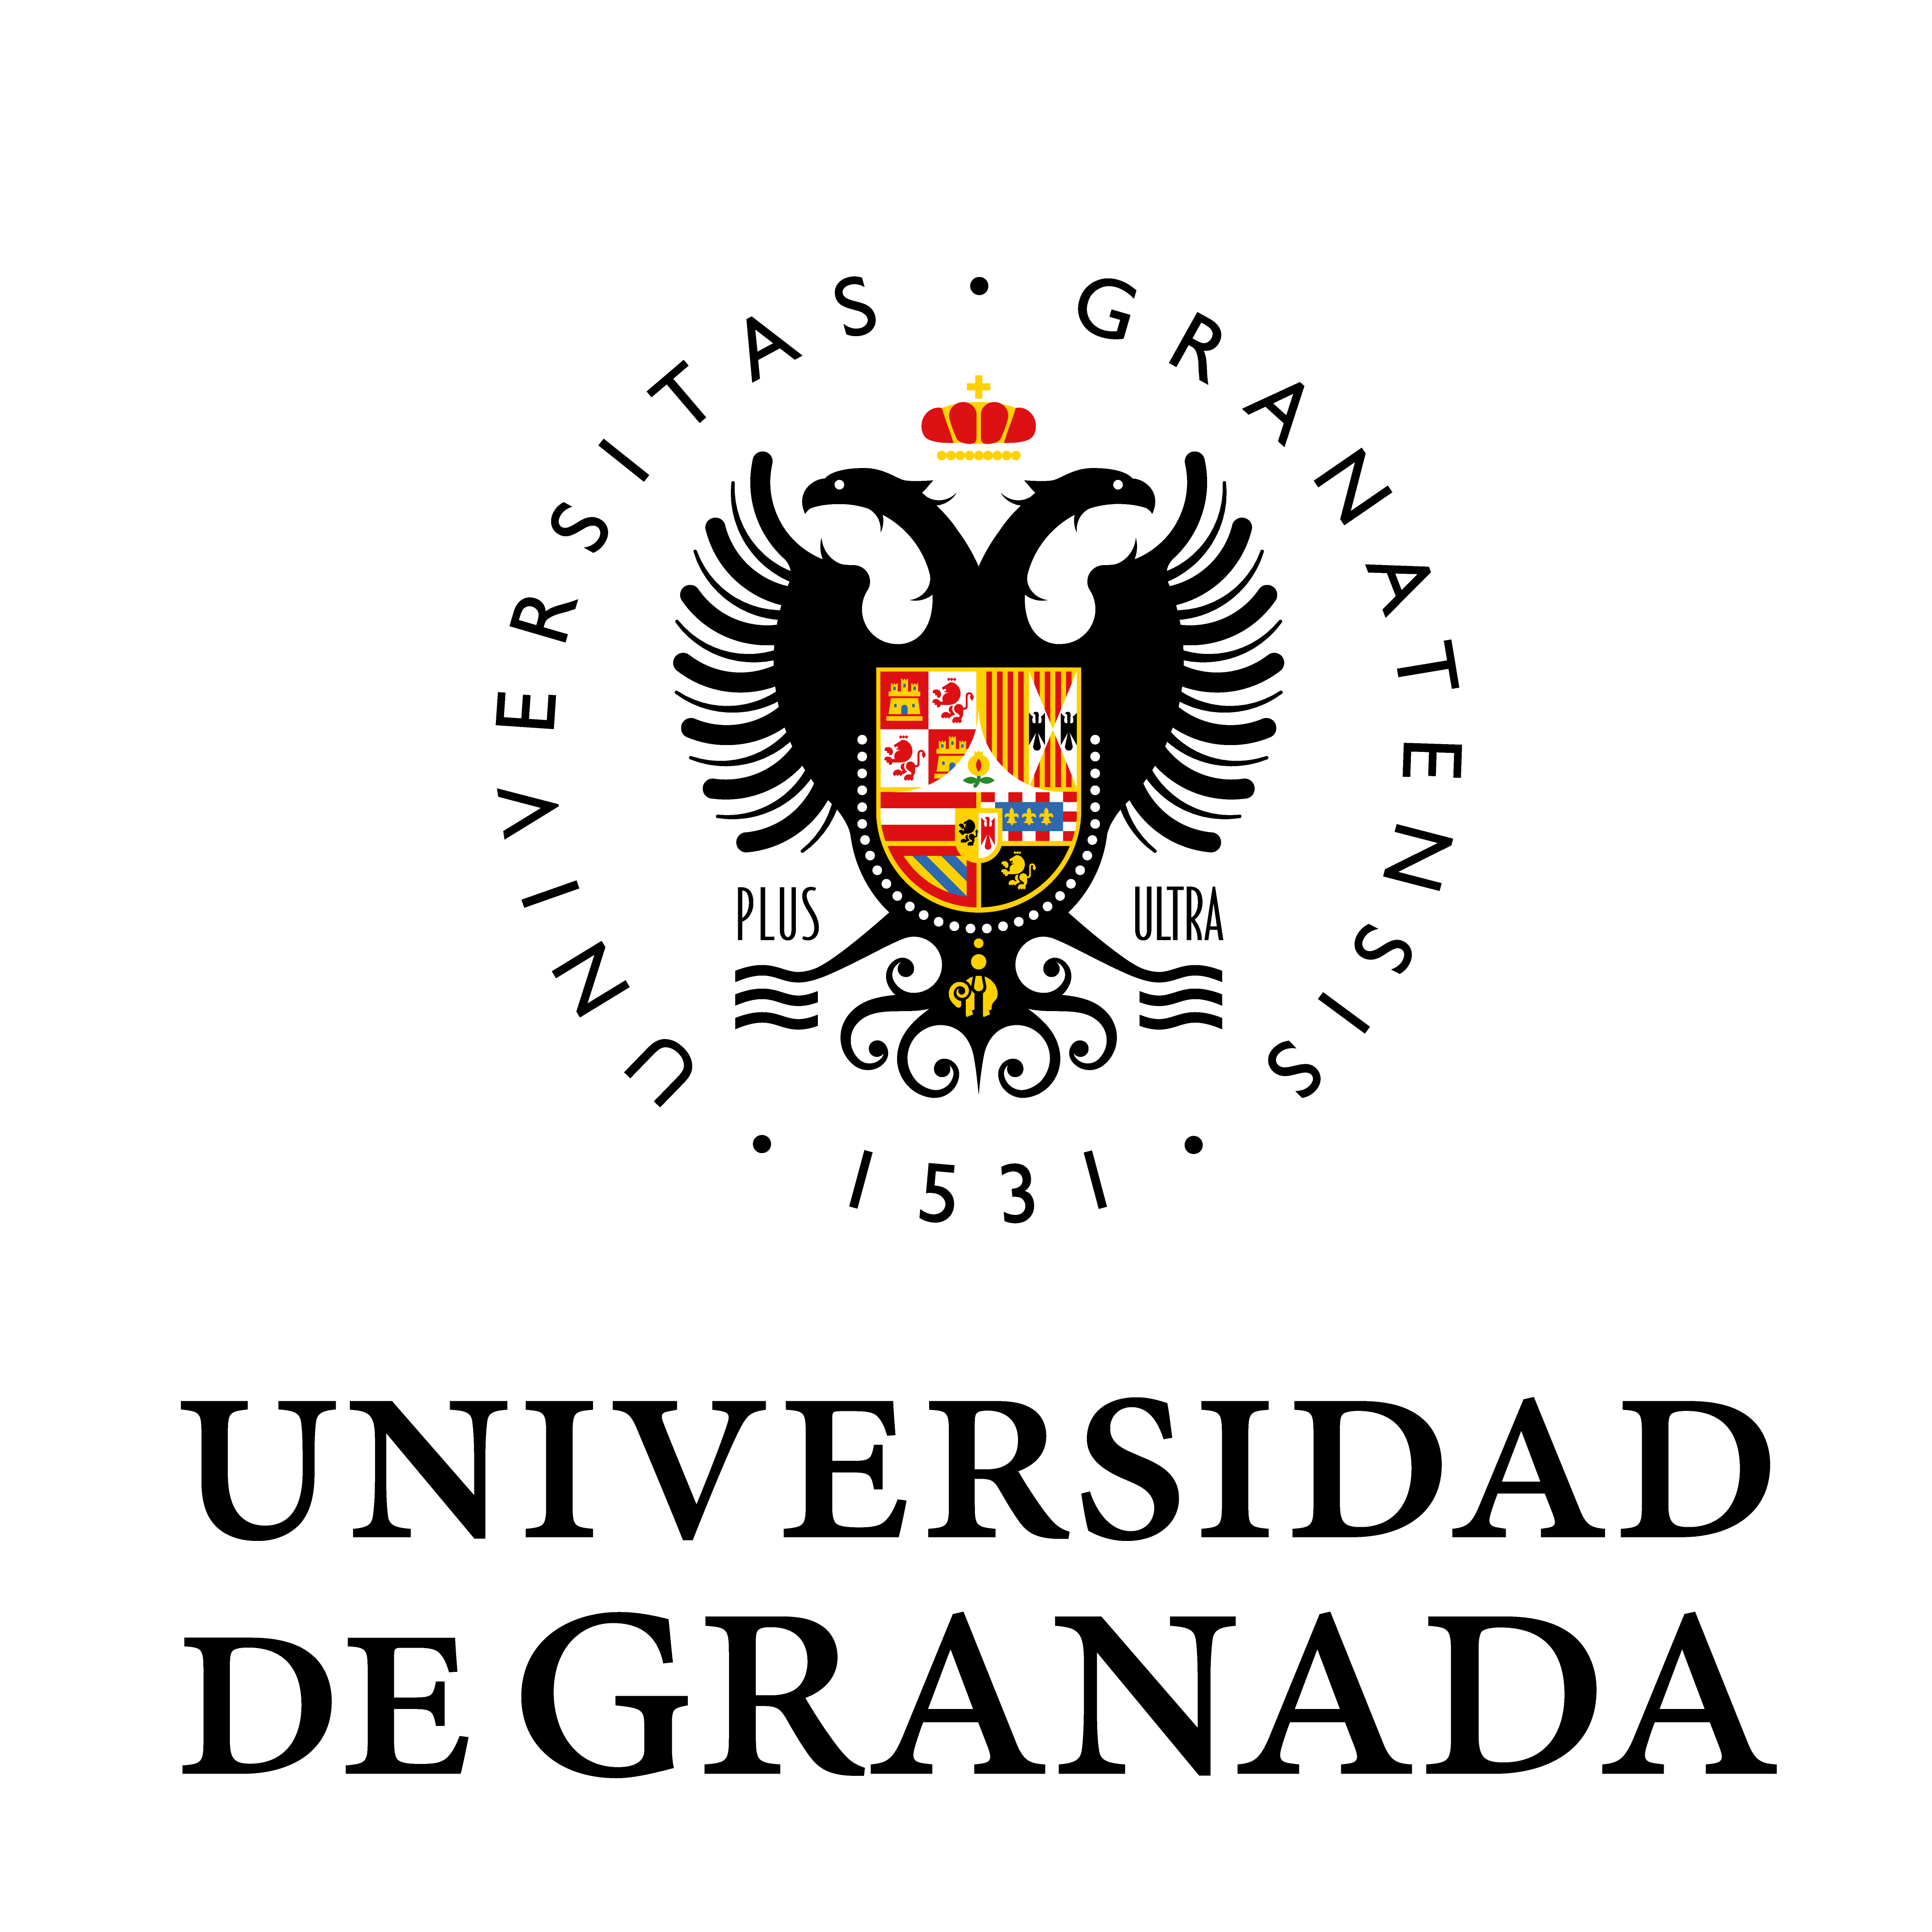
\includegraphics[width=0.4\textwidth]{logo_ugr.png} 
    
    \vspace{2.5cm}
    
    % Datos del autor
    {\large \textbf{Minerva Cebrián Marín} \par}
    \vspace{0.3cm}
    {Grado en Ingeniería Informática + Administración y Dirección de Empresas \par}
    \vspace{0.3cm}
    {Asignatura: Dirección de Recursos Humanos \par}
    
    \vfill % Empuja lo siguiente al final de la página
    
    \large{2025-2026} 
\end{titlepage}

\newpage
\tableofcontents
\newpage

\section{Preguntas de las Tres Lecturas}

\begin{enumerate}[label=\textbf{\arabic*.}, leftmargin=*, topsep=10pt, itemsep=15pt]

    \item \textbf{¿Qué entiende por EMPLOYER BRANDING? Justifique la respuesta.} \\
    Entiendo que el Employer Branding es 
    un conjunto de estrategias y acciones que una empresa utiliza 
    para crear y gestionar su imagen como empleador. El objetivo es 
    atraer y retener a las personas. Ahora, el concepto de Employer
     Branding digital está tomando su lugar, porque si los candidatos 
     tienen una experiencia digital,
     la marca de la empresa como empleador también debe ser digital.

    \item \textbf{Explique cómo esta tendencia puede condicionar la gestión de los recursos humanos de la empresa.} \\
    La forma en que se manejan los recursos humanos está cambiando. 
    Ahora, en lugar de solo controlar, el papel de los departamentos de recursos humanos es 
    ayudar a que las cosas funcionen mejor y brinden un valor real a la empresa.
    Para lograr esto, es importante que se adapten a la forma en que los candidatos buscan 
    empleo y utilizan las redes sociales. Esto significa que todos los procedimientos deben ser digitales.
    También es necesario cambiar la forma en que se capacita y se ofrecen beneficios a los empleados.
     Cada generación tiene diferentes necesidades y expectativas, por lo que no se puede tratar a todos
     de la misma manera.
    Lo más importante es ser coherente. Lo que se dice y lo que se hace deben ser lo mismo.
     Si no, se pierde la confianza de los empleados.

    \item \textbf{Busque 3 ejemplos de empresas catalogadas como “EMPLOYER BRANDING” y explique qué acciones realizan en esa materia.} \\
    
    \begin{itemize}
        \item \textbf{MSD:} Con el proyecto “Está en mí” 
        después de hacer encuestas y grupos de enfoque para saber qué valores 
        tienen en común sus trabajadores. Quieren que todos se sientan orgullosos de trabajar allí. 
        Para lograr esto, decoran los lugares de trabajo de manera especial y participan en certificaciones como Top Employers. 
        El objetivo es atraer a personas capacitadas y talentosas que quieran trabajar con ellos. 
        \item \textbf{Securitas Direct:} Quería que la gente los viera como una empresa innovadora y tecnológica, no solo como una empresa tradicional. Para lograr esto, decidieron trabajar más de cerca
         con escuelas de negocio y universidades. También cambiaron la parte de su sitio web que se dedica 
         al empleo.
        \item \textbf{Banc Sabadell:} Se enfoca en la responsabilidad social corporativa y en crear
         experiencias que hagan que sus empleados se sientan orgullosos de trabajar allí. Un ejemplo es el Trailwalker, una carrera solidaria. De esta manera, 
        los trabajadores pueden proyectar una imagen de marca sólida sin necesidad de gastar mucho dinero. 
    \end{itemize}

    \item \textbf{Aporte propuestas a la dirección de recursos humanos de una empresa para que gestione eficientemente las diferentes generaciones que puedan existir en su plantilla.} \\
    Para gestionar la diversidad generacional, los Recursos Humanos 
    deben crear sistemas de compensación adaptados a cada etapa de la vida. Es clave 
    fomentar el aprendizaje mutuo: jóvenes comparten sus habilidades digitales y veteranos 
    aportan su experiencia.
    Las empresas deben hacer encuestas periódicas para escuchar a sus empleados y ajustar 
    políticas según las necesidades del equipo.
    Para aumentar la motivación, se recomienda fomentar la participación y autonomía en decisiones.
    Para equilibrar vida laboral y profesional, invertir en herramientas de teletrabajo y 
    capacitación virtual es fundamental.
    La dirección debe asegurar una cultura coherente para generar un verdadero sentido de pertenencia.

    \item \textbf{Identifique y justifique los principales retos a los que se van a enfrentar las organizaciones en materia de dirección de recursos humanos.} \\
    El mayor reto es atraer y retener talento valioso. Los trabajadores capacitados tienen una mayor 
    rotación y buscan un sentido de compromiso.Las empresas deben gestionar la diversidad 
    generacional. Deben adaptar sus políticas a las necesidades tecnológicas y valores de cada grupo. El objetivo es que la convivencia en el trabajo impulse la creatividad.
    Para evitar que los nuevos perfiles se aburran, es clave cerrar la brecha motivacional. 
    Esto significa brindar entornos de aprendizaje y autonomía.
    El departamento de Recursos Humanos enfrenta el desafío de cambiar su función. 
    De ser administradores, deben pasar a ser facilitadores estratégicos. Su aporte
    debe tener un valor real para el negocio.
    Además, deben asegurar la coherencia organizacional. Esto implica que lo que la empresa 
    dice debe estar alineado con lo que los empleados viven.
    Por último, deben integrar el Employer Branding digital.
    Esto ayuda a atraer candidatos que valoran la ética y la flexibilidad en el trabajo.

\end{enumerate}

\vspace{1cm}

\section{Pregunta del Bloque ``Lecturas Complementarias''}

\begin{enumerate}[label=\textbf{6.}, leftmargin=*, topsep=10pt]

    \item \textbf{Identifique y justifique las principales tendencias en dirección de recursos humanos a raíz de la pandemia COVID-19.} \\
    
        \begin{itemize}
            \item \textbf{Teletrabajo y modelo híbrido:}La pandemia demostró que trabajar 
            desde casa era posible y daba buenos resultados.
            Sin embargo, hoy en día no todo el mundo trabaja desde casa. Ahora se busca un
             equilibrio entre trabajar en casa y en la oficina.Esto tiene sentido porque une 
             lo mejor de ambos mundos. Ofrece la flexibilidad y libertad que se necesita, 
             al mismo tiempo que mantiene espacios en la oficina para fomentar la cultura de 
             la empresa, la creatividad y que el equipo se lleve bien.
             \item \textbf{Prioridad de la salud y conciliación:} Una tendencia importante es que las personas cambian lo que consideran prioritario
 en el trabajo. Los trabajadores de hoy en día se preocupan mucho por su salud, tanto física como mental, y por sentirse seguros. Quieren encontrar un equilibrio entre el trabajo y su vida personal. Esto significa que los departamentos de Recursos Humanos deben crear políticas que se centren en cuidar a los empleados. De esta manera, podrán atraer y retener a las personas más talentosas. La salud y el bienestar son fundamentales para los trabajadores, y las empresas deben priorizar el cuidado de sus empleados.

            \item \textbf{La digitalización y el uso de datos en Recursos Humanos:}
El Barómetro DCH muestra que la función de Recursos Humanos se ha vuelto más digital porque las
 empresas necesitan gestionar a sus empleados desde cualquier lugar. Ahora, las empresas utilizan 
 tecnología para reclutar, capacitar y comunicarse con sus empleados. Además, cada vez más empresas
  están usando People Analytics y Big Data para tomar decisiones informadas sobre el ambiente laboral 
  y la productividad. Casi el 60 por ciento de las compañías están considerando implementar estas 
  herramientas para tener datos reales que les ayuden a tomar decisiones estratégicas.
\end{itemize}
    

\end{enumerate}

\end{document}